
\item Pacotes tendo massa de \SI{25}{\kilogram} são passados para a calha de escoamento a $v_{A}=\SI{0.9}{\meter/\second}$ utilizando-se uma calha transportadora. Determine suas velocidades quando eles chegam aos pontos $B$, $C$ e $D$. Calcule também a força normal da calha sobre os pacotes em $B$ e $C$. Despreze o atrito e a dimensão dos pacotes.

\import{answers/}{answer-6}

\vspace{-3.6cm}
\begin{flushright}
    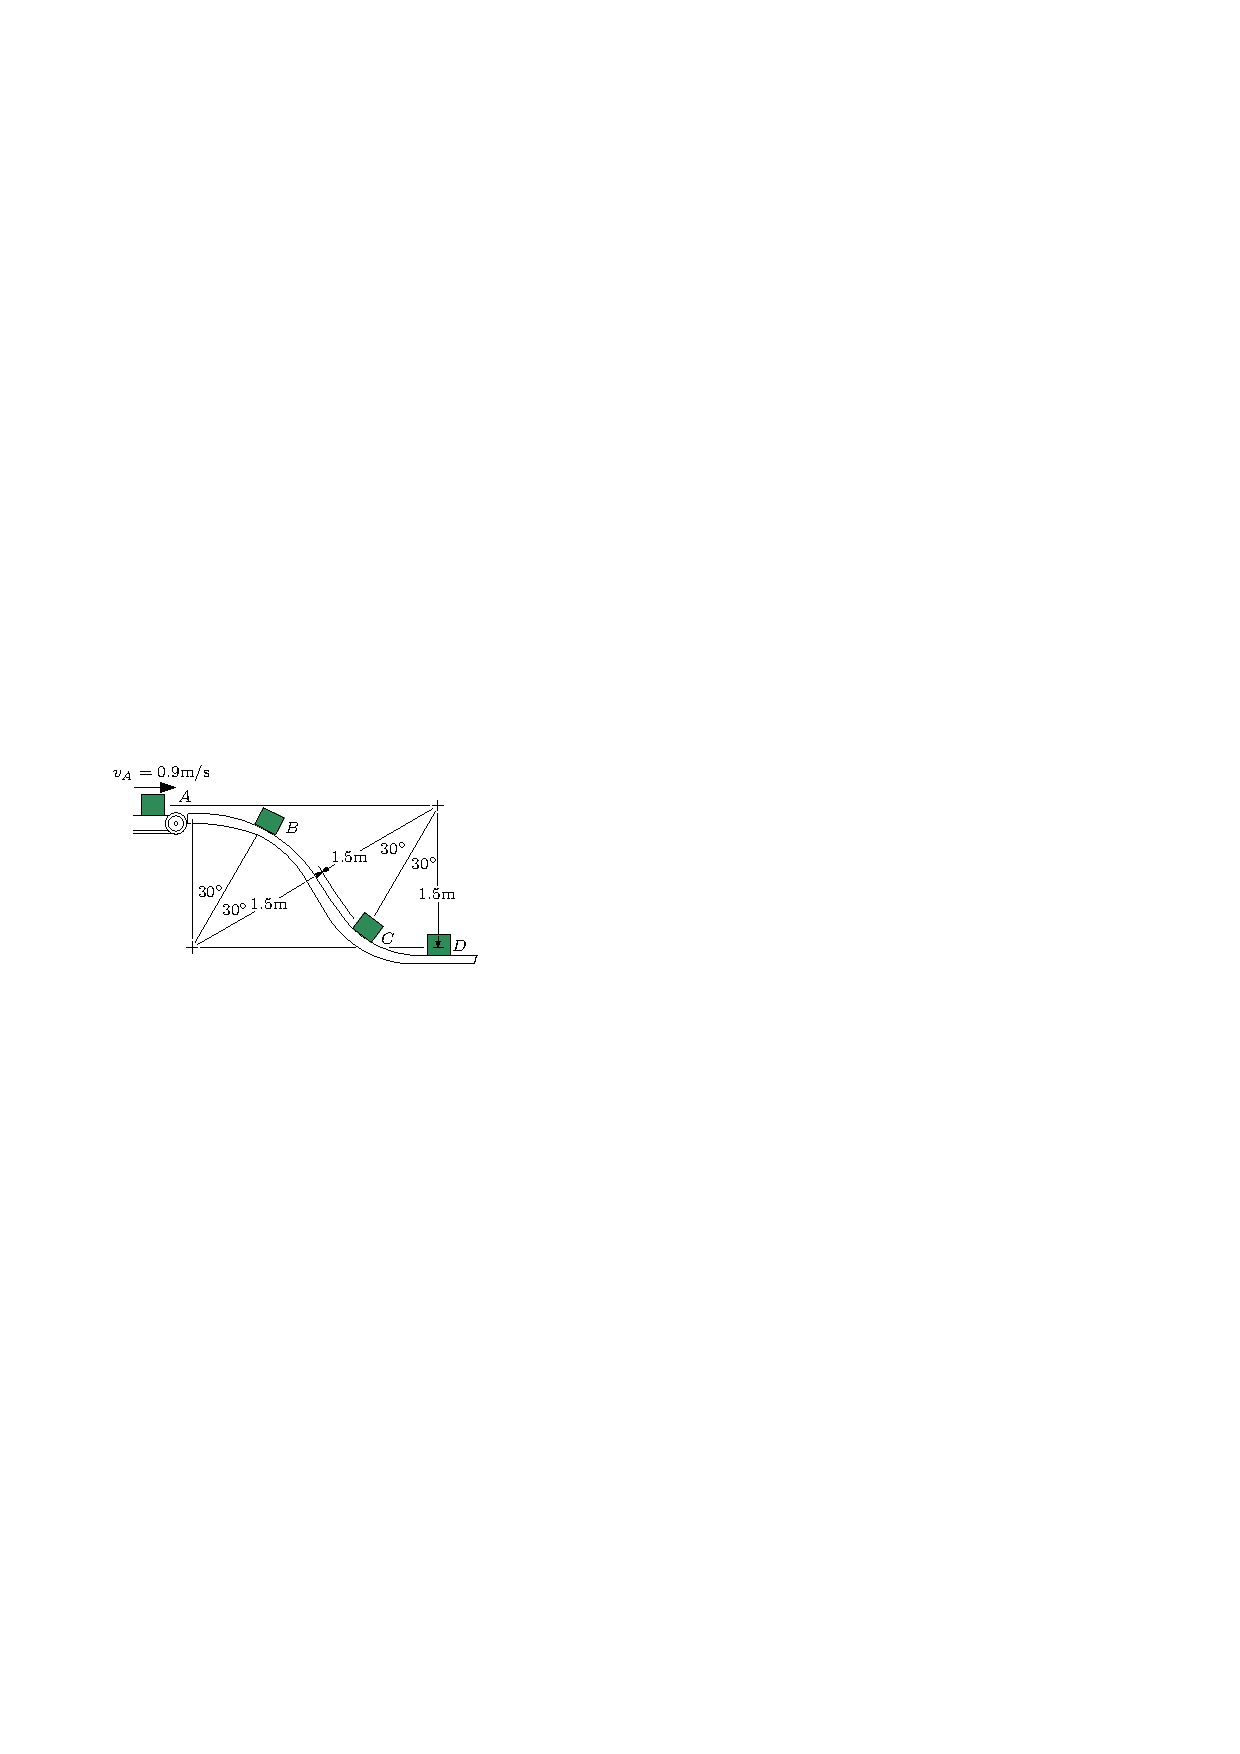
\includegraphics[scale=1.7]{images/draw_6.pdf}
\end{flushright}